\documentclass[10pt,twocolumn]{article}

% use the oxycomps style file
\usepackage{oxycomps}
\usepackage{hyperref}
\usepackage{graphicx}

% read references.bib for the bibtex data
\bibliography{references}

% include metadata in the generated pdf file
\pdfinfo{
    /Title (Comps Proposal)
    /Author (Alec Phillips)
}

% set the title and author information
\title{Comps Proposal}
\author{Alec Phillips}
\affiliation{Occidental College}
\email{aphillips2@oxy.edu}

\begin{document}

\maketitle

\section{Problem Context}

% come back to this section last and give all the context needed to understand the project and the following sections

Software testing is a core principle of computer science that is often overlooked or at least under-emphasized in 
computer science education. Testing is an integral part of any software project, and is a skill that must be developed 
like any other technique in software development. It takes considerable knowledge to be able to develop robust and 
efficient test cases that create confidence in one's code. Thus, this skill should be honed and developed along with 
other programming techniques. Software testing is also nuanced and there are numerous testing techniques that are 
important for students to learn about and have experience putting into practice. The importance of software testing 
serves as the motivation behind my comps project idea; I would like to create a web application that teahches software 
testing and the strategy of test-driven development. 

A web application that teaches software testing would be beneficial to computer science education in general because 
it could be added to a standard computer science curriculum to help students get exposure to the concept. My goal is to 
provide comprehensive materials on software testing as well as hands on exercises where learners can put the concepts 
into practice. Instructors could add this to their curricula, or self-learners could utilize it to gain exposure to 
software testing techniques. 

\section{Technical Background}

This section will cover the relevant terminology that is critical for understanding the technical side of my project as
well as the general goals of my application. These include general software testing techniques, as well as the framework 
of test-driven development. It is also important to distinguish between software testing strategies and software 
development frameworks, and how these concepts interact.

\subsection{Software Testing Techniques}

Testing is a nuanced aspect of software development, and there are several key techniques that are commonly employed for 
writing tests. These different techniques are often used together to comprehensively exercise code, as they work 
together to test a single application in different ways. Thus, it is not sufficient to know just one of these 
techniques; a competent developer should be familiar with all of them, in order to know what to utilize depending on 
their needs. Software testing can be broken up into four main categories depending on the scope and motivation of the 
test. These categories are unit testing, integration testing, end-to-end testing, and acceptance testing 
\cite{Luo2001Article}. These are the four categories of testing that I plan to teach in my application, so it is 
important to elaborate on them in this section. 

Unit tests are those that have the narrowest 
scope. These are tests that apply to individual modules of code. Defining a specific unit of the code is up to the 
developer, but it is standard for unit tests to apply to specific functions, although it can also apply to an entire 
module. Integration testing checks that the individual units are interacting as expected. This means that the interfaces 
between the units as well as the general information flow between them should be exercised. System, or end-to-end 
testing evaluates the overall requirements of the entire application. System tests would generally involve providing 
inputs at the most general or external level, and evaluating that the outputs are as expected. For these tests to pass, 
all the internal processes of the aspect being tested must be functioning correctly. Acceptance testing is the final 
step, in which it is determined if the piece of software conforms to the general specification requirements, and also 
aligns with what the client or user is expecting \cite{Luo2001Article}. 

In addition to the four categories of testing discussed above, there are also two styles of tests that serve different 
purposes, and can each be applied to a either subset or all of the above categories. Once again, it is important to know 
both of these styles, as a thorough test suite should incorporate both. These two types are functional and structural 
testing. Functional is the more broad of the two, in the sense that any of the four categories of tests above can be 
functional in nature. Functional tests are also called 'black box' tests. These tests are ones that assume no knowledge 
of the underlying implementation of the code being tested, and only examine the expectied behavior of the section of 
code being run. These are tests that could be written provided only with the API for a class, or the definition of a 
function, along with an understanding of the expected output. In contrast, structural tests, or 'white box' tests, 
take into account the implementation of the code. They are geared towards exercising specific sections of the 
implementation to make sure that the internal code is operating as expected. This is looking deeper than just expected 
outputs, but instead at the operations taking place within the code. Unit tests, integration tests, and system tests 
can all be structural, however acceptance tests cannot. This is because acceptance tests evaluate whether the system's 
bahavior aligns with what the end user is expecting, and the user or client will (likely) not have any understanding of 
the internal implementation of the code \cite{Sawant2012Article}. My intention is to expose students to both of these 
testing styles in my application.

\subsection{Test-Driven Development}

This section will provide an overview of test-driven development, elaborating on how this software strategy is put into 
practice, its general goals, and how it fits into context with specific testing methods and other software 
development techniques. It is important to understand that test-driven development is not a testing strategy, such as 
the ones discussed in the prior section. Instead, it is a software development framework, meaning
that it informs the entire software development process, not just the testing aspect \cite{George2004Article}. This is 
an important distinction to make, as it is critical to understanding the general aims of test-driven development. This 
section will also discuss some of the benefits and shortcomings of test-driven development. 

Test-driven development lays out a detailed approach to developing software that is centered around allowing 
code testing to push forward the project. The general idea is that test cases are written that in turn motivate the code 
that needs to be written. The general steps in test-driven development are: 1 - write test cases for the next unit of 
code being added to the project, 2 - write the code that the first test case is exercising (until it satisfies the test 
case), 3 - refactor the code as needed, 4 - re-run all existing test cases to check for regressions in the code base 
\cite{Bhat2006Article}. This process then repeats until the project is complete. Thus, this process informs the 
development of the entire project, not just the testing aspect. 

Test-driven development fits within the Agile approach of software development \cite{Janzen2005Article}. Agile 
strategies tend to involve an iterative process that repeats until a project is complete, and is a common industry 
practice. This sits in contrast to older styles of development, such as Waterfall, which have more upfront design 
prior to coding. With Agile methods, design is incorporated into each iteration of development, making thee approaches 
more adaptive. This is beneficial if challenges come up, as design decisions can change more easily as 
needed. With a strategy like Waterfall, where all the design takes place before coding, it becomes more difficult to 
adjust design decisions later on in the project. Test-driven development is also considered a practice of extreme 
programming, or XP, which takes basic development principles, such as testing, and emphasizes them to drive the entire 
development process \cite{Desai2008Article}. 

It is also important to acknowledge that there are downsides to test-driven development. These shortcomings are valuable 
for me to understand before incorporating test-driven 
development as an main aspect of what my application will teach, as well as for users to understand. I do not want to 
present the concept as the ultimate or only way to approach software development, however I believe it is useful for 
students to be exposed to the concept and that it a valuable way for students to learn the importance of software testing. The main 
limitations of test-driven development stem from the fact that there is little emphasis on overall system design 
\cite{George2004Article}. This can necessitate heavy code refactoring later on, since everything is developed in small 
chunks. Thus, it is important that my application conveys the importance of overall system design so that students are 
aware of its importance. I want users of my application to be aware of these considerations, should they choose to practice test-driven 
development in their own projects. 

\section{Prior Work}

There is a considerable amount of existing research into the effectiveness of test-driven development. There have been 
several studies examining test-driven development in industry. This section will use these to get a better sense of the 
concept and its efficacy. Additionally, there is some research into the addition of test-driven development to 
academic curricula. This research will help me evaluate how best to integrate test-driven development into an 
educational application. 

\subsection{Test-Driven Development in Industry}

I looked at two studies exploring the effectivenss of test-driven devlopment in industry. Both of these compared a group 
that used test-driven development and a control group that employed their standard development practices. The first 
study looked at two divisions in Microsoft (Windows and MSN). This study looked at effects of test-driven development on 
code quality as well as total development time. Code quality was calculated by number of code defects as well as 
KLOC (thousands of lines of code) between teams using test-driven development and teams in the control group. 
Using these metrics, the study found that, for both departments, code quality was higher with test-driven development, 
while development time was also higher; the Windows division had 2.6 times higher code quality and the MSN team had 4.2 
times higher code quality using test-driven development, but also experienced 35 and 15 percent increases in development 
time respectively \cite{Bhat2006Article}. It is encouraging that the implementation of test-driven development increased 
code quality, and interesting that it also raised development times. The reason behind this could just be that the 
developers were more accostomed to the workflows of their previous development strategy, so they were slightly slower 
when using test-driven development. However, this difference in efficiency is fairly significant, so it is worth 
considering the balance between code quality and work efficiency. 

The second study took programmers from three companies and had them pair program a bowling game. The programmers were 
split into test-driven development groups and control groups. They were evaluated on their ability to pass a set of test 
cases that they were not allowed to test against before submitting, and also their ability to write their own comprehensive test cases. 
Their time spent to complete the project was also assessed. This study found quite similar results; the test-driven 
development groups passed more of the test cases, but took longer to develop the project by 16 percent 
\cite{George2004Article}. This aligns with the findings in the previous study, and it is interesting that once again the 
test-driven development groups took longer to develop the project than the control groups. However, it is positive that
in both studies, the use of test-driven development seemed to lead to fewer errors. Another interesting finding from this 
study is that all but one of the control groups failed to provide comprehensive test cases for their code, despite being 
directed to do so \cite{George2004Article}. I find this to be particularly interesting, because even professional 
developers chose not to thoroughly test their code when it was not built in as a part of their development process. This 
emphasizes the value of test-driven development's integration of testing into the coding process, because even 
professionals are not always inclined to thoroughly test their code. 

\subsection{Software Testing in Education} 

This section will discuss some of the strategies that have been used to teach software testing and test-driven 
development in the past. This will inform the approach that I take for teaching software testing in my application. 
I came across a significant amount of discussion on the reasons why software testing is undertaught, as well as why 
students find it to be an uninteresting concept to learn. Additionally, there was discussion of how test-driven 
development specifically could be integrated into computer science education. 

The lack of emphasis on software testing in education stems from both students and instructors. Computer science courses 
as well as entire programs are already packed with material, so adding lessons or assignments focused solely on testing 
can be infeasible \cite{Edwards2003Article2}. Additionally, students often find implementation of projects more exciting 
than testing their code, and testing can often appear tedious. Students can also be unmotivated to 
test their code, because they do not want to see it fail \cite{Carrington1997Article}. This is also something that I 
have noticed as a teaching assistant; students will sometimes write test cases that are very specific to their code, 
when more general test cases would not pass. From being a TA I have also noticed that, in general, students do not take 
writing test cases very seriously. Even when instructed to write tests, students in Data Structures will treat it as an 
afterthought, heavily prioritizing other aspects of their projects. 

If the incentives were flipped, and students had 
more of a desire to write failing test cases, they would likely take the task more seriously. This can inform the way 
that I design my practice exercises in the application; instead of having students write code and then test it, I would 
provide them with code that they then need to exercise with test cases, and their performance on this activity will be 
dictated by how robust their tests are. One potential way this could work is by providing a function that fails on some 
edge case which the learner has to identify on their own and then write a test that causes the provided code to fail. 
This would incentivise the student to thoroughly understand both the goal of the function, as well as the actual code, 
and would provide the desire to write a good test that fails the code. 

There is also existing research on having students apply the concepts of test-driven development in order to learn 
computer science in general. This would make software testing a more integral part of every project that students take 
on, shaping the belief that testing is an important part of writing code. Some strategies for implementing this in an 
education setting were to make students fully responsible for demonstrating the correctness of their code 
\cite{Edwards2003Article1}. This would mean that students would not be given any automated test results before 
submitting their code, and would instead be responsible for determining their code's correctness on their own. This may 
be unrealistic to implement in a classroom setting, because it would likely put an even greater strain on students, 
espcially when computer science classes are already time consuming and challenging. However, I can base the exercises in 
my application around this idea, requiring students to write code along with test cases that must reach a certain amount 
of coverage of their code, or catch certain edge cases. 

\section{Ethical Considerations}

An application geared towards education may initially appear to be ethical, however there are still potential moral issues. 
Any application or product geared towards 
users and has the potential to affect real world outcomes has the inherent possibility of affecting negative change. 
Additionally, there are a number of ethical concerns that arise from taking on the role of educator; for instance: what 
are the ethical and pedagogical obligations that an educator has to the students? There is the also the topic of power, as this 
application’s service will likely only affect those who already have 
access to computer science education, reinforcing the current power dynamics in terms of who has access to education and 
the ability to learn computer science. Additionally, it reinforces power dynamics existing around who has internet 
access. Finally, there is the concern of security, as any web application is open to possible attacks, and any service 
that stores user information, as mine likely will, must consider the risk of exposing individuals’ information that they 
have entrusted to you and the service. Despite the initially benign appearance of this project, these ethical 
considerations emphasize that there are still potential ethical issues present that need to be considered carefully. 

\subsection{Educator Obligations}

Taking on the role of educator places one under an ethical burden, as they are entrusted to have expertise on 
the topic and the ability to adequately convey accurate information. The University of Michigan education department 
offers a simple overview of nine core ethical obligations that teachers should uphold. Several of the obligations that 
they bring up will be difficult for me to uphold within the context of this project, specifically
personal responsibility and competence. 

The webpage defines personal responsibility as taking “responsibility for obstacles to student success and to work 
assiduously to ensure equitable access to learning opportunities” \cite{MichiganEducation}. This poses an issue for 
my project because of the amount of time I will be able to dedicate to maintaining this project after it is completed 
and the impersonal nature of an educational application. If this application ends up actually getting deployed, it would 
be infeasible for me to be responsive to every user and their individual needs. 

The article defines competence as “[developing] and continually [working] to improve instructional competence, and to 
strive to engage in professionally-justified teaching practice at all times” \cite{MichiganEducation}. This is 
similarly infeasible because of the commitment that it would take to actively continue improving my instructional 
competence. Within the context of my project, it would require continued updating of the materials and content, as well 
as continuing to further my knowledge to better serve the users of the application, which are not responsibilities that 
I can confidently commit to at this time. These two examples represent the issues that come along with taking on the 
role of educator and building an educational site. In order to address this, it is important that, if this application 
is to be deployed, I only allow it to be active for as long as I can uphold these obligations. 

\subsection{Power Reinforcement}

In addition to the general ethical issues of building an education based application, there is the problem of who will 
have access to this application, and how that reinforces existing power dynamics in the world of computer science and 
technology. Power and computer science are tightly intertwined; technology is nearly omnipresent in our world, and many 
of the most influential and powerful individuals are those who control large technology companies. One clear factor that 
differentiates power in computer science and technology is whether or not someone has 
access to the internet. Individuals who have easy access to the internet are much more easily able to interact with 
existing technologies and web applications, and also have much more access to learning how to interact with computers in 
general. The issue with this web application, and conveying educational material over the internet in general, is that 
it is only making information more accessible to those who can already easily access it. Even if my application makes 
the information easier to learn 
or more enjoyable, it is not reaching a new audience or further distributing access to learning computer science. This 
then reinforces the existing power structures that exist in computer science. 

There is already a large power difference between those who have access to the internet 
and those who do not. The more effective my application is, the more I would be contributing to that power difference. 
The power differences caused by unequal internet access have been well documented, and play a role in global power 
dynamics as well. The advent of the internet has created easy access to information and communication, however this only 
applies to those who have access to it. Societies that do not have the luxury of widespread internet access do not get 
these same benefits, which increases the power differentials between these societies \cite{Fang2018Article}. This 
emphasizes the importance of the relationship between internet access and power. Therefore, further empowering those 
with internet access by means of a web application that only those individuals can benefit from will inherently further 
these existing power dynamics.

Power differences as a result of internet access habe been further exacerbated by the COVID-19 pandemic. This has been a 
prevalent issue in the academic sphere; students 
who have access to reliable internet can more easily and consistently access their courses, and do not have to worry 
about missing material because of something outside of their control like stable internet \cite{Lai2020Article}. 
This emphasizes that, currently, those without internet access are experiencing even greater challenges as a result of 
the pandemic, so introducing more web based applications will further this divide. These issues are important to 
consider, but my hope is that ultimately my application can provide more benefit to individuals and make computer 
science more accesible overall. 

\subsection{Ethics of Security}

This application also brings in the issue of security. The application will likely store user data, such as passwords 
and usernames in a database. If the application is attacked, this user data could be leaked. Additionally, a part of my 
application involves running users' code to evaluate their performance on coding exercises. This brings in the 
possibility of malicious code injection. To ensure that it is ethical to deploy this application, it will be critical 
for me to make sure that I am diligent in securing the 
application from potential attacks such as these, in order to feel confident that my application is not putting anyone's 
information in danger. 

\section{Methods} 

% for the actual comps final paper:
%   - the methods will talk more about the iterative process of testing the app, getting feedback, and then 
%     implementing that into the project
%   - can also include some of the stuff about code design, UI justification, and diagrams of UI webpage/route flow
%   - less stuff about actual code design, especially for server-side & database (this will go on code documentation)

% for the comps proposal paper:
%   - add section at the beginning justifying my UI design
%   - add diagram of UI flow (pages/routing)
%   - add discussion of design specific to test-driven development
%       - how I plan to design exercises to teach this concept (just writing tests, writing code & tests, etc.)
%   - brainstorming of how I could go about the iteration of testing and improving the app
%       - how will I test, what sorts of things would I ask testers

\subsection{Implementation}

The implementation of this project will have three main parts: the front-end code, the server-side code, and the 
database. To build this, I plan to use React, Express, and mySQL. The two most nuanced aspects of the implementation 
will likely be the integration of an in-page text editor and the evaluation of student code from coding exercises. For the 
text editor, I have found a tutorial that I will be using for how to implement this using React. The alternative to this 
approach would be to have users submit files containing their code, instead of having them type directly into an editor 
in the webpage. I would prefer to offer the in-page editor because I think it would be more intuitive for users. 
However, the option of having users submit files is a potential backup if incorporating an editor proves to be rather 
challenging. As for code evaluation, at this point I do not 
have a specific approach for its implementation, but it is at least valuable to 
be aware that this aspect will be challenging. When it comes time to start coding, I will know to prioritize this part 
of the project. 

\subsection{Design}

I would like to allow the application to be interacted with by users with accounts where their progress on materials and
exercises is preserved, as well as by users without accounts, where all the materials and exercises are still accessible 
but their progress is not saved. This is inspired by \href{https://codingbat.com/java}{CodingBat}, which is one of my favorite online computer science 
education resources \cite{CodingBat}. This cite was created by a Stanford professor for his introductory computer 
science students. It offers the option for users to create an account and save their progress, but users who do not wish 
to create an account can still access all of the instructional material. I also find the overall experience of using the 
website to be intuitive and simple. The user interface is bare-bones and easy to navigate. I think the main way 
that I would like my interface design to differ from CodingBat is in the organization of the exercises in relation to 
the supplementary content explanations; I would like to place more emphasis on pairing together the exercises and 
explanations, and also offer a more clear path through the material so that the content can build on itself. A diagram 
of my desired site layout can be found in figure \ref{UI-flow-diagram}.

\begin{figure}[!ht]
    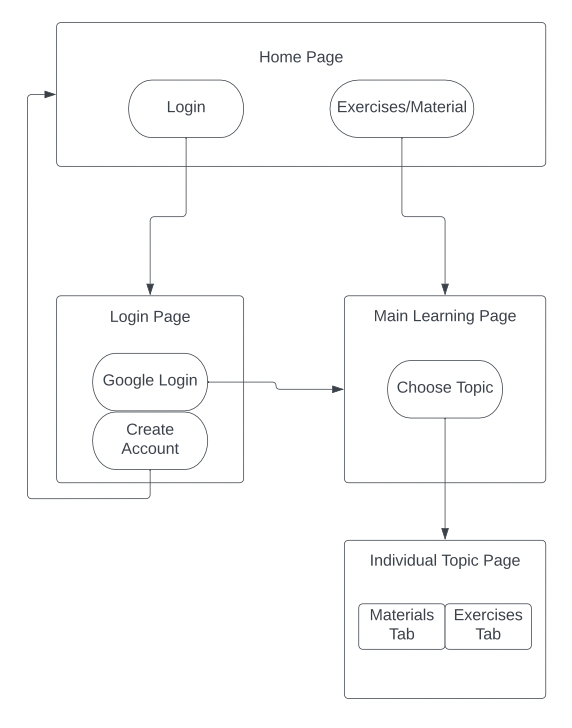
\includegraphics[scale=.7]{./images/UI-Flow-Diagram}
    \caption{Intended Application UI/Page Flow}
    \label{UI-flow-diagram}
\end{figure}

\subsection{Hands on Research}
% TODO: go more in depth on the specific questions that I will ask in these interviews

To inform my decisions for this project, I will conduct interviews with both computer science educators as well as 
industry professionals. This will allow me to get important perspectives on what I should aim to accomplish with my 
application. By interviewing professors, I will have a better sense of what material I should emphasize in order to 
fill in the gaps of what may be missing from computer science curricula regarding software testing. I plan to interview 
the professors in the Occidental computer science department. I would like to ask questions about what aspects of 
computer science testing they think are most important for students to learn, and what materials relevant to software 
testing would best complement their own course content without overlapping with what their students are already 
learning. This way, my application can fit with what instructors are looking for, so that it can be something that 
could get used to accompany a computer science course. 

Through interviewing 
professional software developers, I will be able to see what practices are most important for students to learn before 
entering the industry so that they can be well prepared. Specifically, I would ask questions about what software testing skills are most 
useful for students to have to be prepared for the industry, what styles of software testing are most common, and what 
types of software development strategies are most commonly utilized in a professional setting. This will inform what 
material will be most beneficial for my application to teach. 

\subsection{Iterative Project Improvement}

I plan to
iteratively evaluate and improve my project throughout the semester. This will allow me to get consistent feedback and 
see growth and improvement in my project over time. It would also incentivise me to have a prototype version of the 
application completed early, so that it is more feasible to get actual user testing of the application before the final 
project deadline. To do this, I would like to perform two rounds of evaluation prior to the submission of the 
project (see proposed timeline for specific target dates). For each round, I will perform the survey step, synthesize 
the results, and make appropriate adjustments based on feedback. 

\section{Evaluation}

% for final comps paper (could also do this in this paper too):
%   - discussion of evaluation metrics could actually go before the methods, since it will be useful context since they
%     will get discussed in the methods (how evaluation helped me iteratively improve the project)

% for comps proposal paper:
%   - consider putting eval section before methods
%   - more specific about how i will survey users 
%       - how/where will I get people
%       - what i will have them do
%           - possibly have some who used the app and some who didn't both answer questions & take a short test
%               - could have them write test cases, or reasoning questions about edge cases, etc.

There are several parts of the application that I would like to evaluate independently: 1 - testing the robustness of 
the application in terms of ability to handle user traffic and efficiently evaluate user submissions; 2 - the usability 
of the application in terms of user interface and experience; 3 - the effectiveness of the educational material on the 
application.

\subsection{Robustness}

This is likely the easiest aspect of the project to evaluate, because it can be done without relying on anyone else. I 
can test the efficiency of the code evaluation on my own using Postman to send some large number of requests to the 
system simultaneously. I would like to set benchmarks and see how the system is able to live up to them for different 
numbers of requests. I will have to do some research to figure out exactly what these targets should be, in order to see
what reasonable targets are for performance.

\subsection{Usability}

As opposed to the robustness testing, the user experience  of the application will 
require user-testing. I would like to get at least ten respondents who are computer science majors at Occidental College 
to evaluate this aspect of the project. It is important that they are computer science students, because I will be 
having them evaluate the text editor, and I would like them to have a frame of reference going into this part of the 
evaluation. I will create a Google Form survey that asks respondents to evaluate how 
intuitive and usable the application is. There would be several prompts for the users in order to give them experience using the applicaion 
before responding to the survey questions. First I would prompt them to spend two minutes exploring the application 
freely to get a feel for the organization. Then I would prompt them to navigate to a specific exercise on the website, 
in order for them to assess the difficulty of getting to a particular page they want to get to. This way, they would 
get to see the entire UI flow and see all the pages. Finally, I would ask 
them to try typing into the code editor. The survey questions would have them rank: 1 - their overall impression of how 
intuitive the application layout is, 2 - the difficulty of finding the particular webpage that they were directed to 
find, 3 - the organization of the educational content, 4 - the design of the exercise/material pages, 5 - the visual 
appearance of the text editor (text highlighting and language accuracy), 6 - the experience of 
typing in the editor in terms of responsiveness. Each of these would be ranked on a Likert Scale from 1 to 5. 
Additionally, I would offer an open ended feedback section at the end. This would be valuable during the iterative 
improvement stage so that I can get a sense of what users would like to see improved and what worked well. To analyze 
the data and create visualizations of the evaluations, I would use Google Sheets; the Google Form survey data can be 
sent directly into a Sheet, making this process simple. 

\subsection{Educational Quality}

To evaluate the quality of the educational materials, I would like to get feedback from both computer science students 
as well as computer science professors. First the evaluation of students will be discussed.  I would like to get responses from at least ten Occidental 
College computer science students. Ideally these students would be different from the ones evaluating usability. I 
could choose to combine these aspects of the survey, but I would rather have these surveys remain separate, because I 
would not want the surveys to take a long time to complete or the respondents to experience survey fatigue. The 
participants would be given the link directly to the 'main learning page' of the application and prompted to choose a 
topic to learn. They would be given twenty minutes to read the material and attempt the associated exercise. They would 
then be asked several questions about the experience: 1 - how comprehensive were the material options, 2 - how clear was 
the material explanation, 3 - how clear were the exercise directions, 4 - how difficult was the material to understand, 
5 - how difficult was the coding exercise. Once again, these would use a Likert scale from 1 to 5, and would be analyzed 
in Google Sheets. 

An alternative approach that I was considering was to conduct an experiment in which participants 
complete a short software testing exam that asks conceptual questions about testing and includes a short coding section 
where they are told to write different types of tests for a specific function. I would have a control group that is just 
given the test, and an experimental group that is given access to my application while taking the test. I would then 
compare the scores between the two groups. I opted against this strategy because the outcomes would be highly dependent 
on the prior experience of the participants which would make the results less informative. If I could limit the 
participants to senior computer science majors it could control some of this variability, but I worry that would create 
too small of a participant pool and I would not get a sufficient number of responses. 

I would like to survey at least four computer science professors at Occidental. The professors would be asked to look at 
three lessons of their choice on the application, looking at both the explanations and exercises. They would be asked 
several questions rated on a scale from 1 to 5: how comprehensive are the material options; how clear are the 
explanations; how clear are the exercise directions; would you incorporate this as part of a course. They would also be 
asked several other questions that are rated 
differently: what skill level are the materials appropriate for (introductory, moderate, advanced); what materials would 
you add (open ended). These professor evaluations would provide extremely valuable feedback, as they would have 
considerable insight into computer science education. 

\section{Proposed Timeline}

Summer (tasks to be completed by listed date):

\begin{itemize}
    \item{July 15: Complete interviews with computer science educators. Research and detailed plan for how to implement 
    the code exercise evaluation mechanism within my application.}
    \item{August 30: Complete interviews with industry professionals. Complete design specification for application
    based on information gathered from interviews.}
\end{itemize}

Fall Semester:

\begin{itemize}
    \item{September 15: All server-side and database code complete, including code evaluation mechanism.}
    \item{October 1: All client-side (React) code complete and integrated with server-side code. This constitutes a 
    complete prototype for the project.}
    \item{October 15: First round of user testing complete.}
    \item{November 1: Integration of first user evaluations complete, ready for second round of evaluations.}
    \item{November 15: Second round of user testing complete.}
    \item{December 1: Integration of second user evaluations complete.}
    \item{Final Deadline: Completion of final comps paper.}
\end{itemize}

\printbibliography 

\end{document}
